%%%%%%%%%%%%%%%%%%%%%%%%%%%%%%%%%%%%%%%%%
% Short Sectioned Assignment
% LaTeX Template
% Version 1.0 (5/5/12)
%
% This template has been downloaded from:
% http://www.LaTeXTemplates.com
%
% Original author:
% Frits Wenneker (http://www.howtotex.com)
%
% License:
% CC BY-NC-SA 3.0 (http://creativecommons.org/licenses/by-nc-sa/3.0/)
%
%%%%%%%%%%%%%%%%%%%%%%%%%%%%%%%%%%%%%%%%%

%----------------------------------------------------------------------------------------
%	PACKAGES AND OTHER DOCUMENT CONFIGURATIONS
%----------------------------------------------------------------------------------------

\documentclass[titlepage, paper=a4, fontsize=11pt]{scrartcl} % A4 paper and 11pt font size

\usepackage[T1]{fontenc} % Use 8-bit encoding that has 256 glyphs
\usepackage{fourier} % Use the Adobe Utopia font for the document - comment this line to return to the LaTeX default
\usepackage[english]{babel} % English language/hyphenation
\usepackage{amsmath,amsfonts,amsthm} % Math packages
\usepackage{listings}

\usepackage{lipsum} % Used for inserting dummy 'Lorem ipsum' text into the template
\usepackage{graphicx}


\usepackage{sectsty} % Allows customizing section commands
\allsectionsfont{\centering \normalfont\scshape} % Make all sections centered, the default font and small caps

\usepackage{fancyhdr} % Custom headers and footers
\pagestyle{fancyplain} % Makes all pages in the document conform to the custom headers and footers
\fancyhead{} % No page header - if you want one, create it in the same way as the footers below
\fancyfoot[L]{} % Empty left footer
\fancyfoot[C]{} % Empty center footer
\fancyfoot[R]{\thepage} % Page numbering for right footer
\renewcommand{\headrulewidth}{0pt} % Remove header underlines
\renewcommand{\footrulewidth}{0pt} % Remove footer underlines
\setlength{\headheight}{13.6pt} % Customize the height of the header

\numberwithin{equation}{section} % Number equations within sections (i.e. 1.1, 1.2, 2.1, 2.2 instead of 1, 2, 3, 4)
\numberwithin{table}{section} % Number tables within sections (i.e. 1.1, 1.2, 2.1, 2.2 instead of 1, 2, 3, 4)

\setlength\parindent{0pt} % Removes all indentation from paragraphs - comment this line for an assignment with lots of text

%----------------------------------------------------------------------------------------
%	TITLE SECTION
%----------------------------------------------------------------------------------------

\newcommand{\horrule}[1]{\rule{\linewidth}{#1}} % Create horizontal rule command with 1 argument of height

\title{	
\normalfont \normalsize 
\textsc{University of Virginia} \\ [25pt] % Your university, school and/or department name(s)
\horrule{0.5pt} \\[0.4cm] % Thin top horizontal rule
\huge ECE/CS 5565 Homework 3 \\ % The assignment title
\horrule{2pt} \\[0.5cm] % Thick bottom horizontal rule
}

\author{Shawn (Shuoshuo) Chen\\sc7cq@virginia.edu} % Your name

\date{\normalsize\today} % Today's date or a custom date

\begin{document}

\maketitle % Print the title

%----------------------------------------------------------------------------------------
%	PROBLEM 3
%----------------------------------------------------------------------------------------

\section*{Problem 3}

Sum of first two 8 bits: 01010011 + 01100110 = 10111001 \\
Sum  with the third 8 bits: 10111001 + 01110100 = 00101110 \\
So its 1's complement is: 11010001 \\
Taking 1's complement for the sum is because at the receiver, when adding all 16-bit words
including the checksum, the result expected should be all 1's. If a bit is 0, that indicates there
are errors. \\

All 1-bit errors will be detected because otherwise the sum will contain 0. But 2-bit errors are
not guaranteed to be detected, for example, a bit is flipped in the data portion and another bit
flipped in checksum. In this case, the sum would still be straight 1's.
\\


%----------------------------------------------------------------------------------------
%	PROBLEM 6
%----------------------------------------------------------------------------------------

\section*{Problem 6}
If the sender sends a packet with sequence number 1, and receiver confirms with an ACK 1.
But the ACK is corrupted when it reaches the sender. The sender then resends packet 1. However,
according to the FSM, receiver has already been waiting for packet 0. As a consequence, it rejects
the resent packet 1 with NAK back to the sender. The sender keeps sending packet 1 and the receiver
keeps rejecting. Both sides go into a deadlock state.
\\


%----------------------------------------------------------------------------------------
%	PROBLEM 8
%----------------------------------------------------------------------------------------
\section*{Problem 8}
Please see Figure \ref{fig:rdt3}.
\begin{figure}[!ht]
    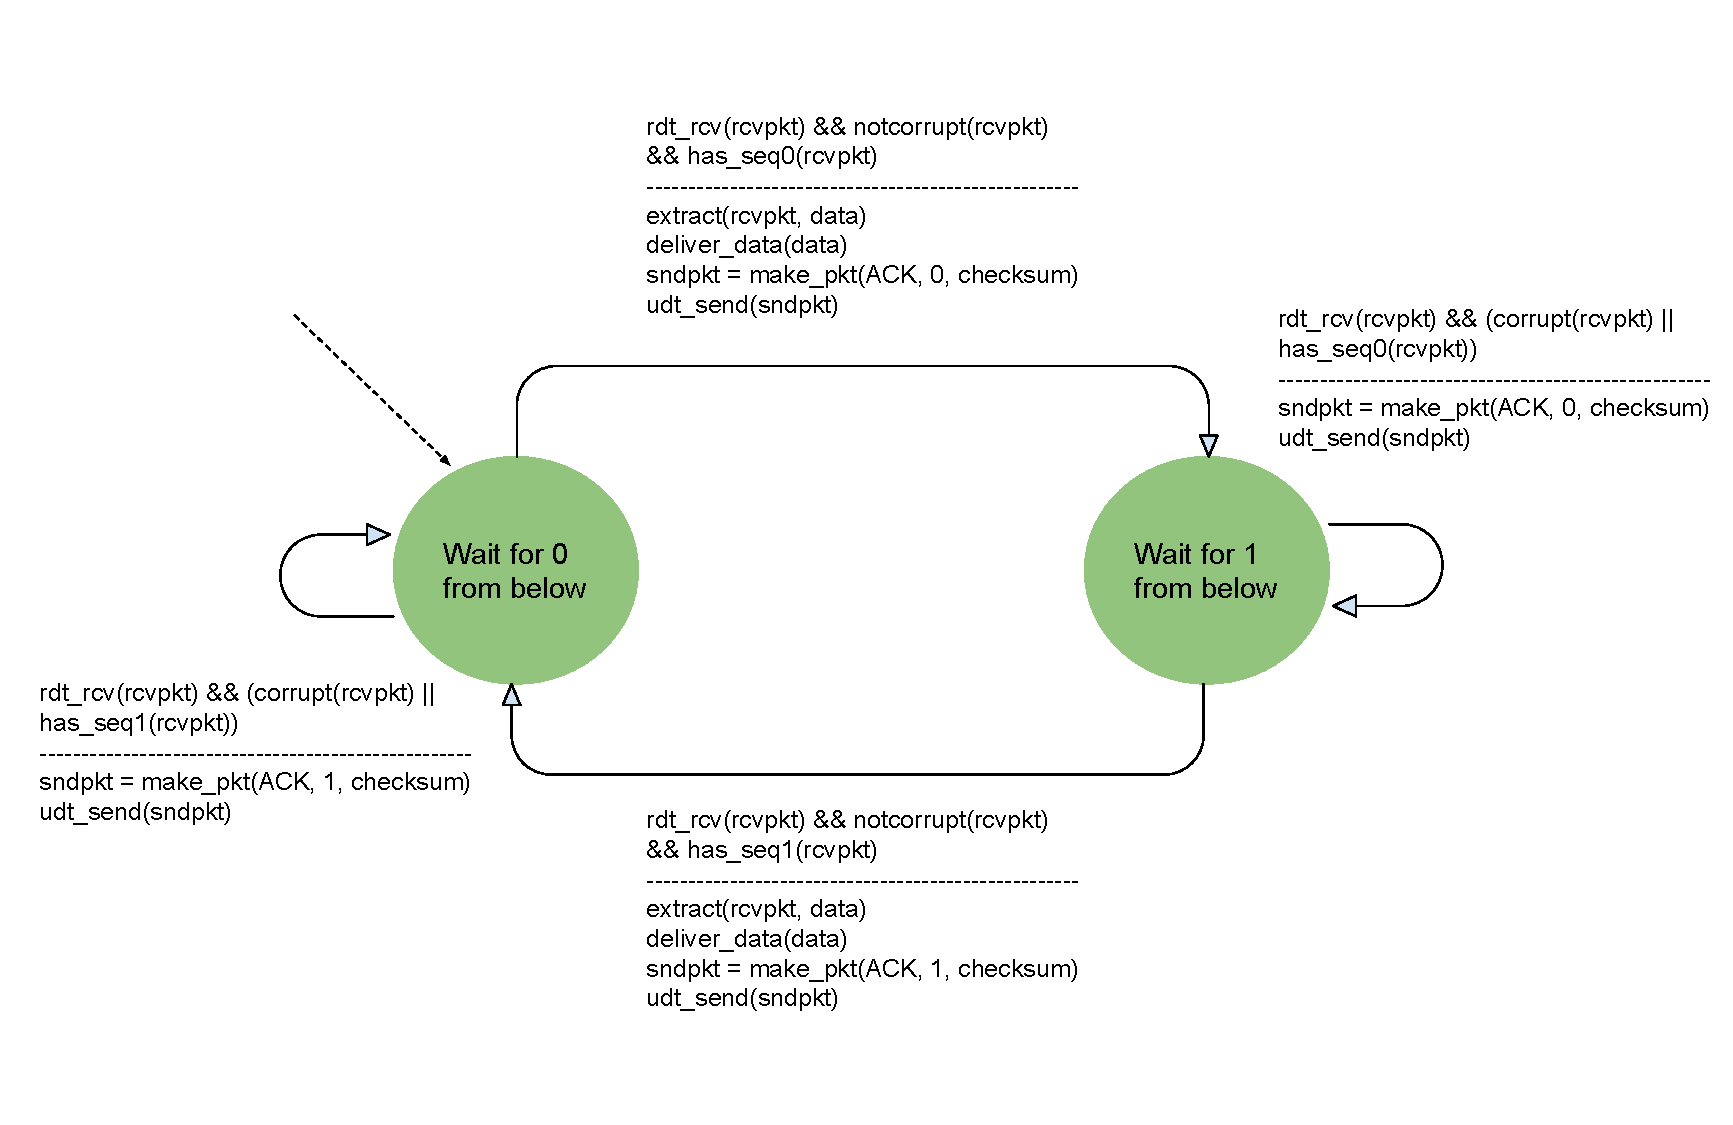
\includegraphics[width=\textwidth]{images/rdt3-rcv-FSM.pdf}
    \caption{Receiver FSM for rdt3.0}
    \label{fig:rdt3}
\end{figure}



%----------------------------------------------------------------------------------------
%	PROBLEM 11
%----------------------------------------------------------------------------------------

\section*{Problem 11}
If the receiver does not send back an ACK and the packet is corrupted, the sender will keep waiting until eventually an ACK shows up.
However, this is impossible to happen. And the receiver also keeps waiting until sender sends something
new. Thus, both the sender and receiver will enter a deadlock state. \\

Similarly, if there is no Wait-for-0-from-below self transition, same thing would happen and both sender
and receiver will enter a deadlock state.
\\

\newpage

%----------------------------------------------------------------------------------------
%	PROBLEM 12
%----------------------------------------------------------------------------------------

\section*{Problem 12}
The protocol will still work, but it would probably cause a huge amount of retransmission. \\
Imagine the timer is premature, thus it goes off before the first ACK comes back. An extra copy of
the packet is sent. Then if bit error occurs causing the ACK to be corrupted, another extra copy of the packet will be sent again. So in the worst case, a packet could be sent 3 times plus the number of ACKs for previous packets on the way.
\\


%----------------------------------------------------------------------------------------
%	PROBLEM 13
%----------------------------------------------------------------------------------------

\section*{Problem 13}
As figure \ref{fig:p13} shows, the first D0 is reordered and appears right before the new D0.
This would confuse the receiver since receiver might take the reordered D0, which it has already received,
as the new D0 expected.
\begin{figure}[!ht]
    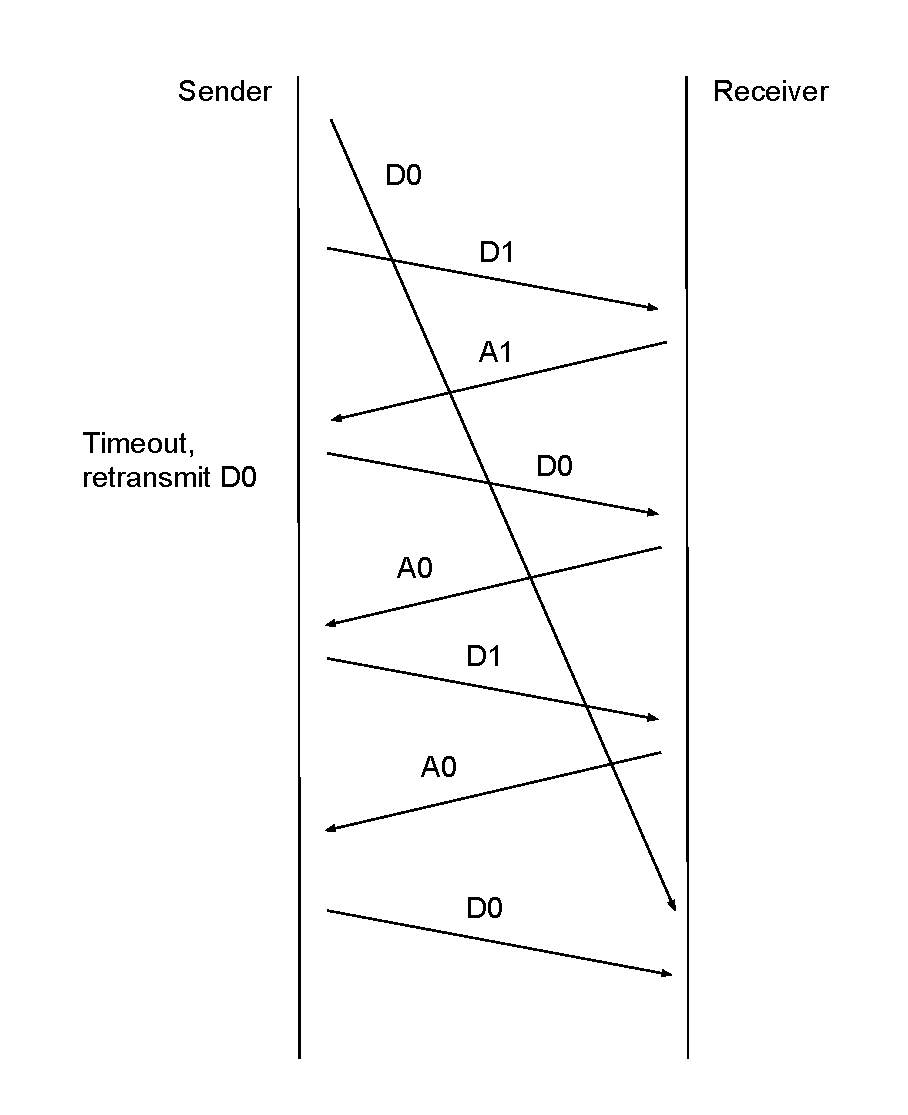
\includegraphics[width=\textwidth]{images/P13.pdf}
    \caption{Out-of-sequence problem}
    \label{fig:p13}
\end{figure}
\\


%----------------------------------------------------------------------------------------
%	PROBLEM 7
%----------------------------------------------------------------------------------------

\section*{Problem 9}
(a). $\Delta$ is the transmission delay on the access link:
\begin{align*} 
\begin{split}
\Delta &= \frac{L}{R} \\
&= \frac{850,000 \  bits}{15,000,000 \  bps} \\
&= 0.0567 \quad seconds
\end{split}					
\end{align*}
The the average access delay can be calculated as:
\begin{align*} 
\begin{split}
T_{access} &= \frac{\Delta}{1-\Delta\beta} \\
&= \frac{0.0567}{1-0.0567 \times 16} \\
&= 0.61 \quad seconds
\end{split}					
\end{align*}
So the total average response time is:
\begin{align*} 
\begin{split}
T_{total} &= T_{access} + T_{Internet} \\
&= 0.61 + 3 \\
&= 3.61 \quad seconds
\end{split}					
\end{align*}

(b). Since a cache in installed in the LAN, only $40\%$ of the requests will go into the Internet,
so the $T_{access}$ now becomes:
\begin{align*} 
\begin{split}
T_{access} &= \frac{\Delta}{1-\Delta \times (0.4\beta)} \\
&= \frac{0.0567}{1-0.0567 \times (0.4 \times 16)} \\
&= 0.089 \quad seconds
\end{split}					
\end{align*}
For the missed requests, total average response time is:
\begin{align*} 
\begin{split}
T_{total1} &= T_{access} + T_{Internet} \\
&= 0.089 + 3 \\
&= 3.089 \quad seconds
\end{split}					
\end{align*}
For the hit requests, total average response time equals transmission delay because
$t_{proc}, t_{queue} and t_{prop}$ can all be ignored. Thus:
\begin{align*} 
\begin{split}
T_{total2} &= t_{trans} \\
&= \frac{L}{R} \\
&= \frac{850,000}{100,000,000} \\
&= 0.0085 \quad seconds
\end{split}					
\end{align*}
Finally, do a weighted average to get the overall average response time:
\begin{align*} 
\begin{split}
T_{total} &= 0.4 \times T_{total1} + 0.6 \times T_{total2} \\
&= 0.4 \times 3.089 + 0.6 \times 0.0085 \\
&= 1.2407 \quad seconds
\end{split}					
\end{align*}
\\


%----------------------------------------------------------------------------------------
%	PROBLEM 8
%----------------------------------------------------------------------------------------

\section*{Problem 13}
MAIL FROM in SMTP is used for the SMTP server to know whom the sender is. It needs to be a valid
email address recognizable by the SMTP server. The From filed is just a human-readable text in the message body.
\\


%----------------------------------------------------------------------------------------
%	PROBLEM 9
%----------------------------------------------------------------------------------------

\section*{Problem 22}
For client-server model, the minimum distribution time can be calculated by:
\begin{align*} 
\begin{split}
D_{cs} &= max\{ \frac{NF}{u_s}, \frac{F}{d_{min}} \}
\end{split}					
\end{align*}
For P2P model, the minimum distribution time can be calculated by:
\begin{align*} 
\begin{split}
D_{P2P} &= max\{ \frac{F}{u_s}, \frac{F}{d_{min}}, \frac{NF}{u_s + \sum \limits{i=1}^N u_i} \}
\end{split}					
\end{align*}
For client-server model:
\begin{table}[h!]
  \begin{center}
    \label{tab:table1}
    \begin{tabular}{ l | l | c | r }
      N/u & 300 Kbps & 700 Kbps & 2 Mbps \\
      \hline
      10 & 7500 sec & 7500 sec & 7500 sec \\
      \hline
      100 & 50000 sec & 50000 sec & 50000 sec \\
      \hline
      1000 & 500000 sec & 500000 sec & 500000 sec \\
    \end{tabular}
  \end{center}
\end{table}
\\
For P2P model:
\begin{table}[h!]
  \begin{center}
    \label{tab:table1}
    \begin{tabular}{ l | l | c | r }
      N/u & 300 Kbps & 700 Kbps & 2 Mbps \\
      \hline
      10 & 7500 sec & 7500 sec & 7500 sec \\
      \hline
      100 & 25000 sec & 15000 sec & 7500 sec \\
      \hline
      1000 & 45455 sec & 20548 sec & 7500 sec \\
    \end{tabular}
  \end{center}
\end{table}
\\


%----------------------------------------------------------------------------------------
%	PROBLEM 10
%----------------------------------------------------------------------------------------

\section*{Problem 23}
(a). The server sends the file to each receiver in parallel with the same rate of $\frac{u_s}{N}$.
Since $\frac{u_s}{N} \leqslant d_{min}$, each receiver can receive at the speed of $\frac{u_s}{N}$.
Thus, the distribution time is the reception time of each receiver:
\begin{align*} 
\begin{split}
D_{cs} &= \frac{F}{\frac{u_s}{N}} \\
&= \frac{NF}{u_s}
\end{split}					
\end{align*}

(b). The server sends the file to each receiver in parallel with the same rate of $d_{min}$.
Because $\frac{u_s}{N} \geqslant d_{min}$, each receiver can only receive at full speed, which is $d_{min}$.
And since all receivers are receiving in parallel, the total time equals the single reception time:
\begin{align*} 
\begin{split}
D_{cs} &= \frac{F}{d_{min}}
\end{split}					
\end{align*}

(c). For $\frac{u_s}{N} \leqslant d_{min}$, there is $D_{cs} \geqslant \frac{NF}{u_s}$.
And for $\frac{u_s}{N} \geqslant d_{min}$, there is $D_{cs} \geqslant \frac{F}{d_{min}}$.
Thus, given any $u_s$, there is $D_{cs} \geqslant max\{ \frac{NF}{u_s}, \frac{F}{d_{min}} \}$.
\\


%----------------------------------------------------------------------------------------
%	PROBLEM 11
%----------------------------------------------------------------------------------------

\section*{Problem 27}
Peer 3 will ask its first successor, peer 4, for the identifier and IP address of peer 4's immediate successor.
Since peer 5 has left, peer 4 is aware and thus makes its second successor, peer 8, its new first successor.
When peer 3 asks peer 4, it returns the information of peer 8. Peer 3 then takes peer 8 as its new second successor.
\\


%----------------------------------------------------------------------------------------
%	PROBLEM 12
%----------------------------------------------------------------------------------------

\section*{WebSocket vs HTTP}
(a). Time-sensitive applications like online games and stock tickers tend to generate data at a high frequency.
In this sense, HTTP long polling and streaming would not be very suitable because the server can only send data
upon client's request. For exmaple, in terms of HTTP long polling and streaming, the stock tickers are generated at the scale of micro seconds while network delay is usually milliseconds. When the client receives a previous response and issues a new request right away, due to network delay, quite a lot of hitorical tickers would be missed since server only returns the latest status. However, WebSocket does not have this problem because upon the update of a tick, server can push it to the client. Even though the ticks are generated at high speed, server is doing pipelining to push the data. No data will be missed. \\

(b). WebSocket and HTTP are actually unrelated. The only relationship is that websocket's handshake is sent to port 80 and interpreted by a web server as upgrade request. The difference between them is that websocket is truly full-duplex, the server can push data to the client. While HTTP is not truly full-duplex though server push can be implemented by HTTP long polling or streaming. \\

WebSocket runs on top of TCP. It establishes a single persistent TCP connection at the handshake phase.
\\


\end{document}
